\cotefile{37}
\scanpage{18}
\margin{\handwritten{\unsure{1.93|1.23}, \unsure{1.27}, 2.9 à reporter au \unsure{3.1}}}

SGA 4 VI

\uline{Sommaire}
\margin{\handwritten{\uline{pp}}}

1. Conditions de finitude pour les objets et flèches d'un topos.\margin{\handwritten{1 à 19}}

2. Conditions de finitude pour un topos.\margin{\handwritten{20 à 37}}

3. Conditions de finitude pour un morphisme de topos. \deleted{\handwritten{\unsure{Cas des limites inductives}}}\margin{\handwritten{38 à 46}}

\deleted{4. Constructibilité.}\inserted{\handwritten{4. Conditions de finitude pour un topos \inserted{obtenu par} recollement.}}\margin{\handwritten{47 à 65}}

\deleted{5}\handwritten{\unsure{6}}. Catégories fibrées et $\underset{\handwritten{\longrightarrow}}{\mathrm{Lim}}$ (rappels).

\deleted{\unsure{6}}\handwritten{7}. Sites et topos fibrés.

\deleted{\unsure{7}}\handwritten{8}. Limites projectives de topos.

\deleted{\unsure{7|8}}\handwritten{\unsure{9|8}}. Cas des limites projectives filtrantes de topos cohérents par morphismes de transition cohérents: théorèmes de passage à la limite pour la cohomologie.
\margin{\handwritten{$\left\{\vphantom{\begin{matrix}a\\b\\c\end{matrix}}\right.$}}

% The curved relocation stroke links the circled replacement number to the position after item 4.
\figure{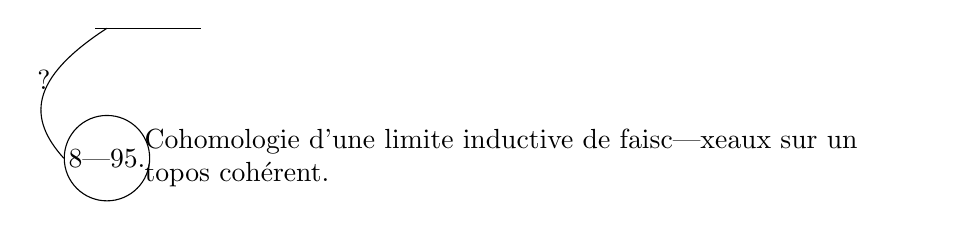
\begin{tikzpicture}[x=0.5cm,y=0.5cm]
\node (a) at (-1.6,2) {\handwritten{\unsure{?}}};
\node[draw,circle,inner sep=1pt] (b) at (0,0) {\deleted{\unsure{8|9}}\handwritten{5}.};
\node[anchor=west,text width=0.82\linewidth,inner sep=2pt] at (0.8,0) {Cohomologie d'une limite inductive de fais\unsure{c|x}eaux sur un topos cohérent\unsure{.}};
\draw (b.west) .. controls (-2,1) and (-2,2) .. (0,3.3);
\draw (-0.3,3.3)--(2.4,3.3);
\end{tikzpicture}}

\handwritten{10. Appendice (par P. Deligne). \deleted{\unsure{Existence de points}} \unsure{d'un|Un} topos cohérent \unsure{a} \inserted{\unsure{suffisamment} de points}.}

\deleted{NB Bien sûr 8 serait interchangeable avec le bloc \deleted{4}\handwritten{5} à \deleted{\unsure{7|8}}\handwritten{\unsure{9}}. Mais il me semble plus naturel de mettre dans deux numéros consécutifs les deux facettes du passage à la limite en cohomologie. Bien sûr, le numéro 8 sera réduit à une ou deux pages, le sorite des conditions de finitude étant déjà fait.}

\deleted{Le n\textsuperscript{o} 4 contiendra le sorite des groupes constructibles (au sens groupes finis ou non), des faisceaux de torsion, des notions de constructibilité pour les Modules et complexes de Modules, - y compris les faits spéciaux dans le cas localement noethérien. Je pense que je le rédigerai mais ne le garantis pas. On peut \deleted{\unsure{à la rigueur}} laisser tomber le n\textsuperscript{o}4, ce sera alors moins beau bien sûr ...:}

\deleted{La rédaction qui suit des n\textsuperscript{o}s 1 à 3 est \unsure{àomplète|complète}, à cela près que je compte y ajouter encore quelques exemples (en particulier un topos localement algébrique non algébrique)\unsure{,|.} \deleted{un morphisme non cohérent de topos cohérents).}}
\inserted{\handwritten{et un topos ayant une famille génératrice formée d'objet\unsure{s} cohérents, qui n'est pas localement algébrique}}
% archive sheet number: 17
